\documentclass[conf]{new-aiaa}
%\documentclass[journal]{new-aiaa} for journal papers
\usepackage[utf8]{inputenc}

\usepackage{graphicx}
\usepackage{amsmath}
\usepackage{commath}
\usepackage[version=4]{mhchem}
\usepackage{siunitx}
\usepackage{longtable,tabularx}
\usepackage{float}
\usepackage{listings}
\usepackage{pdfpages}
\usepackage{color} %red, green, blue, yellow, cyan, magenta, black, white
\definecolor{mygreen}{RGB}{28,172,0} % color values Red, Green, Blue
\definecolor{mylilas}{RGB}{170,55,241}
\setlength\LTleft{0pt} 

\lstset{language=Matlab,%
	basicstyle=\footnotesize,
	breaklines=true,%
	morekeywords={matlab2tikz},
	keywordstyle=\color{blue},%
	morekeywords=[2]{1}, keywordstyle=[2]{\color{black}},
	identifierstyle=\color{black},%
	stringstyle=\color{mylilas},
	commentstyle=\color{mygreen},%
	showstringspaces=false,%without this there will be a symbol in the places where there is a space
	numbers=left,%
	numberstyle={\tiny \color{black}},% size of the numbers
	numbersep=9pt, % this defines how far the numbers are from the text
	emph=[1]{for,end,break},emphstyle=[1]\color{red}, %some words to emphasise
	%emph=[2]{word1,word2}, emphstyle=[2]{style},    
}

% ================================================================ % 
\title{ASE 389P.4 Methods of Orbit Determination \\ Homework 5: Setting Up the Term Project}

\author{Junette Hsin}
\affil{Masters Student, Aerospace Engineering and Engineering Mechanics, University of Texas, Austin, TX 78712}

\begin{document}

\maketitle

\begin{abstract}
	The theory and algorithms are derived and computer program to establish the trajectory of
	an Earth-orbiting satellite is developed. The assumptions for the study are:
	
	\begin{itemize}
		\item Three tracking stations taking apparent range and range-rate data are available for tracking the	satellite. Apparent quantities imply that the one-way light time between signal transmission and	reception were modeled into the measurement (i.e. the effect is dealt with).
		\item The force model used to generate the truth is the EGM96 gravity field of degree and order 20,
		attitude-dependent solar radiation pressure, and atmospheric drag.
		\item The satellite is a box-wing shaped with one Sun-pointed solar panel with known component sizes, material properties, and orientation. The spacecraft -Z axis (in the spacecraft body reference frame) is always Nadir-pointed and has the antenna.
	\end{itemize}
	

\end{abstract}


% ================================================================ % 
\section*{Problem}

% \subsubsection*{Statement} 
\begin{center}
\fbox{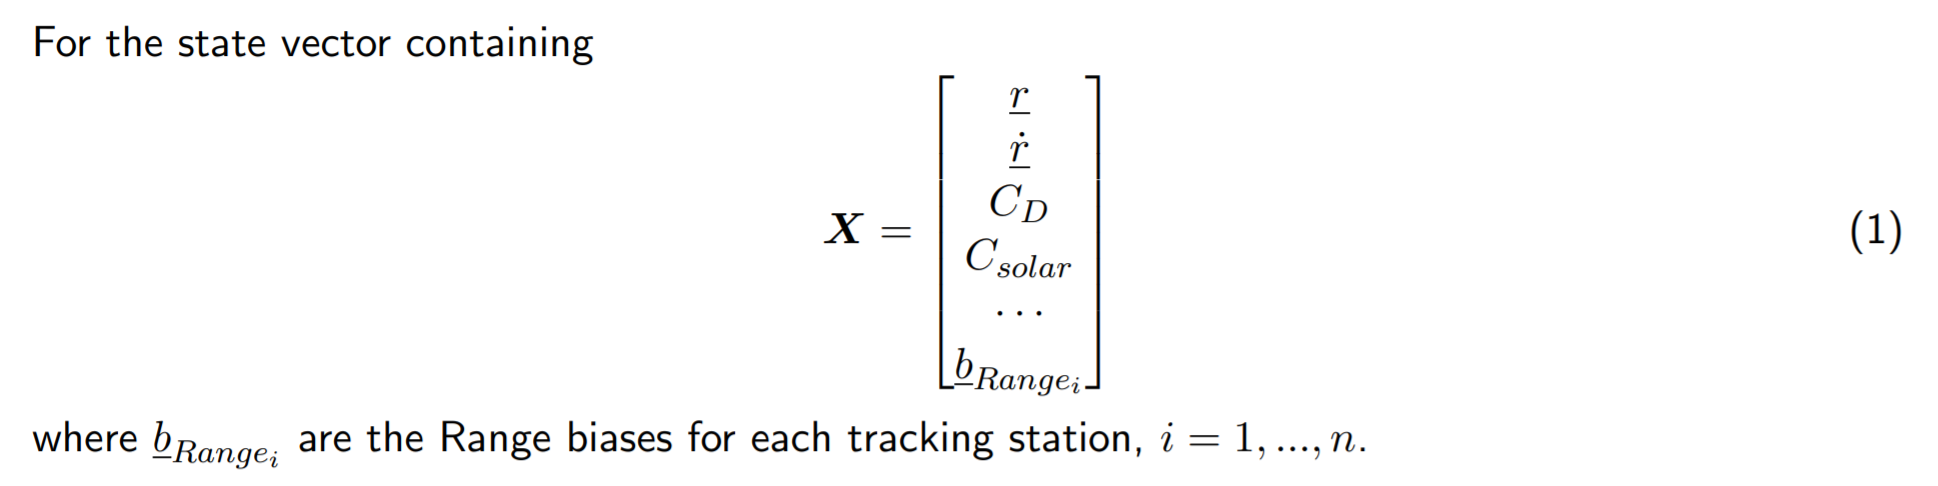
\includegraphics[width=0.9\textwidth]{prob.png}} \\
\end{center}


% ================================================================ % 
\section*{Problem 1}

 % \subsubsection*{Statement} 
\begin{center}
\fbox{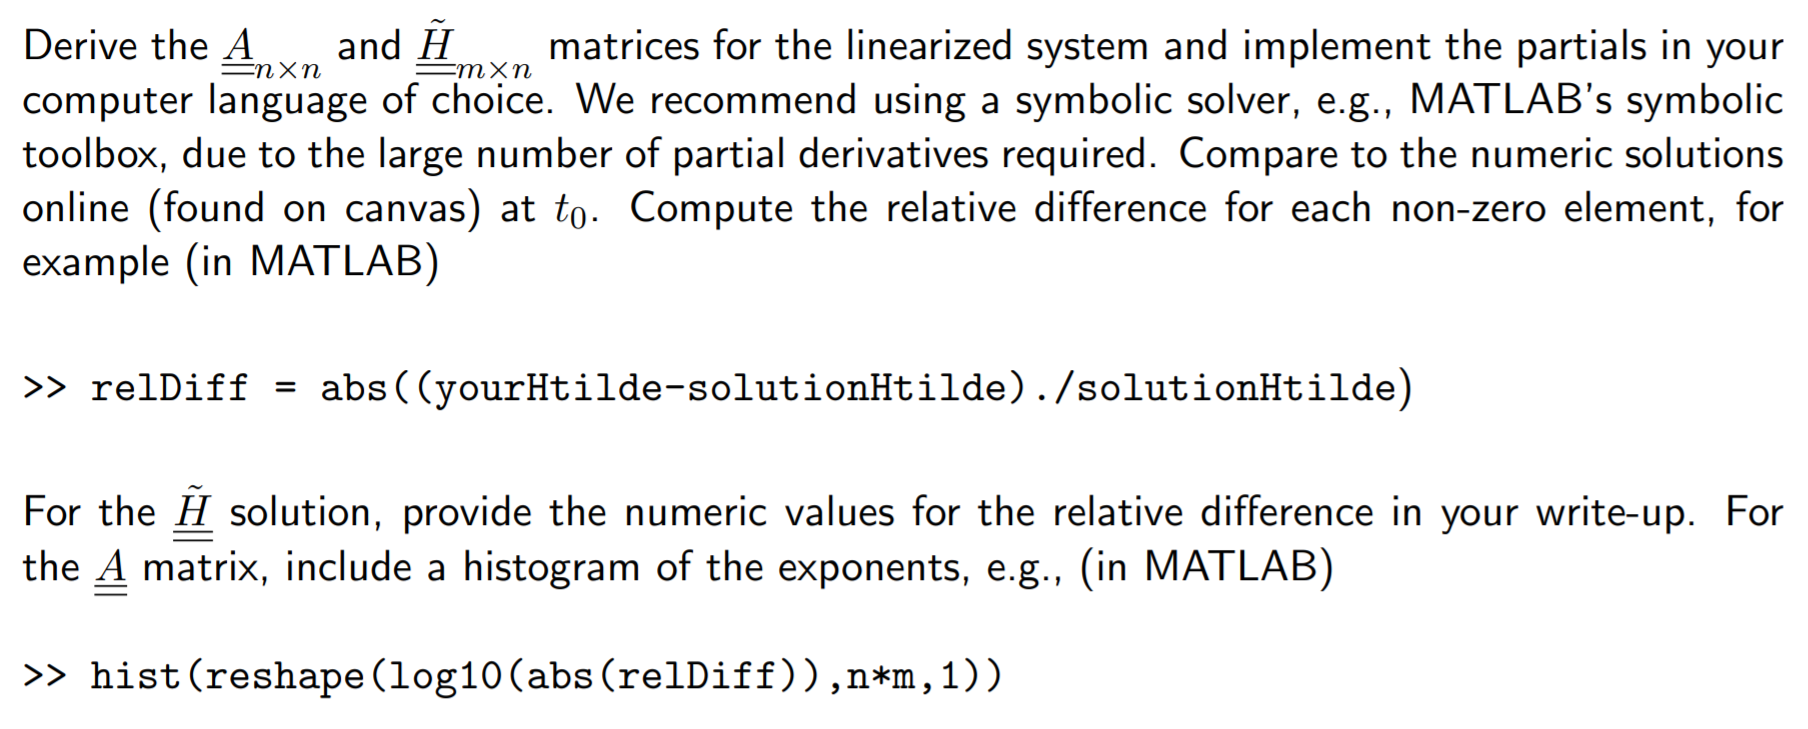
\includegraphics[width=0.9\textwidth]{prob_1.png}} \\
\end{center}

% ---------------------------------------------------------------- % 
\subsubsection*{Solution} 




\newpage
% ================================================================ % 
\section*{Appendix} 

\subsection*{HW4 MATLAB code} 

\begin{lstlisting}[basicstyle=\footnotesize]
% HW 5

\end{lstlisting}



% ================================================================ % 

\bibliography{sample}

\end{document}
